\section{Adeline}

\subsection{Aufbau}

Im 1959 entwickelten der Stanford Professor Bernard Widrow und der Elektroingeneur Marcian Edward Hoff das sogenannte \emph{Adilne-Modell}. Der Name ist ein Akronym für \emph{ADAptive LINear Element}. Dieses Modell basiert auf dem Perceptron mit dem Unterschied, dass dieses Modell auf die Einheits-Sprungfunktion, wie sie das Peceptron verwendet, bei der Angleichung der Gewichte verzichtet. Es wird stattdessen eine lineare Aktivierungsfunktion $g(\mathbf{z})$ verwendet welche in diesem Fall erstmal mit der Identitätsfunktion besetzt wird (es gilt also $g(\mathbf{w}^T\mathbf{x}) = \mathbf{w}^T\mathbf{x}$). Außerdem wird eine Entscheidungsfunktion an das Ende des ganzen Modells gehängt um weiterhin die Werte quantifizieren zu können. Diese hat jedoch keinen Einfluss auf den Trainingsalgorithmus. 

\begin{figure}[!htb]
	\centering
	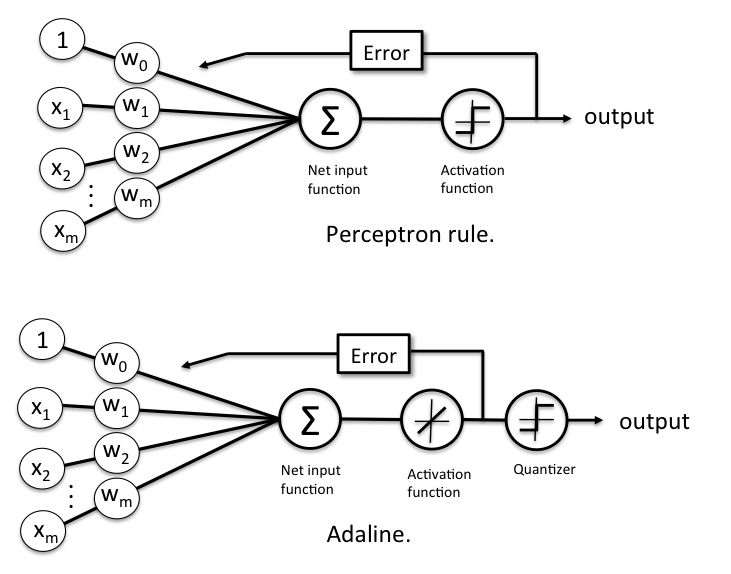
\includegraphics[width=\linewidth]{img/adeline_aufbau}
	\mycaption{Adeline - Aufbau}{mpNeuron}
	\label{fig:ad_aufbau}
\end{figure}


\subsection{Lernregel}

Widrow und Hoff definierten die Delta-Regel für den Lernalgorithmus ihres Modells. Dieser ist auch unter dem Namen \emph{Least-Mean-Square-Algorithmus} bekannt und ist auch heute noch von Relevanz). Im Kern móchte man hierbei das Minimum einer Kostenfunktion über dem Modell bestimmen. Ich werde im folgenden Abschnitt darauf eingehen wie dieser funktioniert und wie genau er für dieses Modell eingesetzt werden kann. 

todo Intro nochmal überarbeiten...

\paragraph{Gradient Descent}
Der wesentliche Nachteil der Einheits-Sprungfunktion ist der, dass sie nicht stetig und und damit nicht differenzierbar ist. Deswegen hat man sich beim Lernalgorithmus des Adeline-Modells dazu entschieden stattdessen die Identitätsfunktion zu verwenden. Es wird zuerst eine Kostenfunktion $J(\mathbf{w})$ definiert die minimiert werden soll. Die Kostenfunktion wird durch die \emph{Regressionsquadratsumme} \footnote{engl. \emph{sum of squared errors} (SSE)} definiert. Die Formel sieh folgendermaßen aus: 

\begin{equation}
J(\mathbf{w})  = \frac{1}{2} \sum_{i} (\text{target}^{(i)} - \text{output}^{(i)})^2 \quad \quad \text{output}^{(i)} \in \mathbb{R} \\
\end{equation}

Wichtig hierbei, der Vorfaktor $ \frac{1}{2} $ gehört nicht zur herkömmlichen Regressionsquadratsumme, wurde hier jedoch hinzugefügt um später einfach ableiten zu können. 


